\chapter{បន្ទុកអគ្គិសនី និងដែនអគ្គិសនី}
\section{អគ្គិសនីកម្ម}
\begin{definition}
	\emph{\kml អគ្គិសនីកម្មៈ} ជាអំពើដែលធ្វើឲ្យអង្គធាតុមួយមានបន្ទុកអគ្គិសនី ពោលគឺធ្វើឲ្យវាលើស ឬខ្វះអេឡិចត្រុង។
	\begin{itemize}
		\item បើអង្គធាតុមួយលើសអេឡិចត្រុង វាផ្ទុកបន្ទុកអគ្គិសនីអវិជ្ជមាន។
		\item បើអង្គធាតុមួយខ្វះអេឡិចត្រុង វាផ្ទុកបន្ទុកអគ្គិសនីវិជ្ជមាន។
	\end{itemize}
\end{definition}
\begin{remark}
	គេបែងចែកអគ្គិសនីកម្មជាបីប្រភេទគឺ អគ្គីសនីកម្មដោយកកិត អគ្គិសនីកម្មដោយប៉ះ និងអគ្គិសនីកម្មដោយឥទ្ធិពល។
\end{remark}
\section{អាតូម និងបន្ទុកអគ្គិសនី}
\begin{itemize}
	\item \emph{\kml អាតូម}
	\begin{definition}
		\emph{\kml អាតូមៈ} គឺជាភាគល្អិតតូចបំផុតនៃរូបធាតុដែលមានលក្ខណៈដូចរូបធាតុដែរ។ រូបធាតុមួយមានប្រភេទអាតូមតែមួយគត់។
	\end{definition}
	\begin{example}
		កាបូនផ្សំឡើងដោយអាតូបកាបូន មាសផ្សំឡើងដោយអាតូមមាស។
	\end{example}
	\begin{multicols}{2}
		\quad អង្គធាតុទាំងអស់ផ្សំឡើងដោយម៉ូលេគុល។ \\ក្នុងម៉ូលេគុលមានភាគល្អិតតូចៗជាច្រើន ហៅថាអាតូម។ នៅចំណុចកណ្តាលនៃអាតូមនីមួយៗមានណ្វៃយ៉ូ ដែលនៅក្នុងនោះមានប្រូតុង និងណឺត្រុង។ នៅជុំវិញណ្វៃយ៉ូនោះមានអេឡិចត្រុងធ្វើចលនាឥតឈប់ឈរ។ ប្រូតុង និងអេឡិចត្រុងផ្ទុកបន្ទុកអគ្គិសនីប្រភេទខុសគ្នា។
		\begin{figure}[H]
			\centering
			\begin{tikzpicture}
			\begin{scope}[scale=0.7]
			\def\proton(#1,#2){%
				\shade [ball color=blue!50] (#1,#2) circle (10pt);
				\node at (#1,#2) {\texttt{$+$}};
			}
			\def\neutron(#1,#2){%
				\shade[ball color=orange!80!red] (#1,#2) circle (10pt);
			}
			\def\electron{%
				\shade[ball color=gray!30] (0,0) circle (8pt);
				\node at (0,0) {\texttt{$-$}};
			}
			\neutron(0.8,0.2)
			\proton(0.5,-0.5)
			\neutron(-0.25,-0.5)
			\neutron(0.55,0.8)
			\proton(-0.5,0.2)
			\proton(-0.1,0.8)
			\proton(0.5,0)
			\proton(0.12,0.6)
			\proton(0.12,-0.6)
			\neutron(-0.25,0)
			\draw[
			postaction=decorate,
			decoration={markings, 
				mark=at position 0.5 with {\electron},
				mark=at position 1 with {\electron}
			}] 
			(0,0) circle (2cm);
			\draw[
			postaction=decorate,
			decoration={markings, 
				mark=at position 0.3 with {\electron},
				mark=at position 0.55 with {\electron},
				mark=at position 0.85 with {\electron},
				mark=at position 0.75 with {\electron}
			}] 
			(0,0) circle (3cm);
			\end{scope}
			\end{tikzpicture}
			\caption{ទម្រង់នៃអាតូម}
		\end{figure}
	\end{multicols}
	\item \emph{\kml បន្ទុកអគ្គិសនី}
	\begin{definition}
		\emph{\kml បន្ទុកអគ្គិសនីៈ}​គឺជាលក្ខណៈមូលដ្ខានមួយ(លក្ខណៈអគ្គិសនី) នៃរូបធាតុដែលកើតមានលើអង្គធាតុជាក់លាក់ មួយចំនួន។
		\quad គេចែកបន្ទុកអគ្គិសនីជាពីរប្រភេទគឺ បន្ទុកអគ្គុិសនីវិជ្ជមាន​ និងបន្ទុកអគ្គិសនីអវិជ្ជមាន។
	\end{definition}
	\item \emph{\kml អេឡិចត្រុង និងប្រូតុង}
	\begin{definition}
		\begin{itemize}
			\item [$-$] \emph{\kml អេឡិចត្រុងៈ} ជាធាតុបន្ទុកអគ្គិសនីដែលមានបន្ទុកអគ្គិសនីអវិជ្ជមាន។
			\item [$-$] \emph{\kml ប្រូត្រុងៈ} ជាធាតុបន្ទុកអគ្គិសនីដែលមានបន្ទុកអគ្គិសនីវិជ្ជមាន។
		\end{itemize}
	\end{definition}
	\begin{center}
		\begin{tabular}{ |c|c|c|c| } 
			\hline
			\text{\DS ធាតុបន្ទុកអគ្គិសនី} & \text{\DS អេឡិចត្រុង} & \text{\DS ប្រូតុង} & \text{\DS ណឺត្រុង} \\
			\hline
			\text{បន្ទុកអគ្គិសនី} & \text{$q_{e}=e^{-}=-1.60\times10^{-19}C$} & \text{$q_{p}=1.60\times10^{-19}C$}​ & \text{$q_{n}=0$} \\ 
			\text{ម៉ាស} & \text{$m_{e}=9.11\times10^{-31}Kg$} & \text{$m_{p}=1.673\times10^{-27}Kg$} & \text{$m_{n}=1.675\times10^{-27}Kg$}\\			
			\hline
		\end{tabular}
	\end{center}
	\item \emph{\kml អំពើនៃបន្ទុកអគ្គិសនី ឬលក្ខណៈនៃបន្ទុកអគ្គិសនី}
	\begin{remark}
		\begin{enumerate}[m]
			\item បន្ទុកអគ្គិសនីដែលមានប្រភេទដូចគ្នា ដាក់ជិតគ្នាវាច្រានគ្នាចេញ។
			\item បន្ទុកអគ្គិសនីដែលមានប្រភេទខុសគ្នា ដាក់ជិតគ្នាវាទាញគ្នាចូល។
		\end{enumerate}
	\end{remark}
	\begin{generality}
		អាតូមនីមួយៗ មានចំនួនអេឡិចត្រុងស្មើនឹងចំនួនប្រូតុងរបស់វាទាំងអស់ដែលធ្វើឲ្យអាតូមណឺតតាមន័យអគ្គិសនី។ ប៉ុន្តែ អេឡិចត្រុងឋិតនៅស្រទាប់ក្រៅដែលដាច់ចេញពីអាតូមដោយកកិត។
	\end{generality}
	\item \emph{\kml រូបមន្តបរិមាណបន្ទុកអគ្គិសនីរបស់ណ្វៃយ៉ូនៃអាតូមៈ} \fbox{$q=Ze$} ដែល $Z$ ជាលេខលំដាប់នៃអាតូម។
	\item \emph{\kml រូបមន្តបរិមាណបន្ទុកអគ្គិសនីនៃអង្គធាតុដែលលើស ឬខ្វះអេឡិចត្រុងៈ} \fbox{$q=\pm ne$}\\
	ដែល $-n$ ប្រើចំពោះអង្គធាតុដែលលើសអេឡិចត្រុង និង $+n$ ប្រើចំពោះអង្គធាតុដែលខ្វះអេឡិចត្រុង។
	\item \emph{\kml រូបមន្តបរិមាណបន្ទុកអគ្គិសនីនៃចរន្តថេរ $I$ ឆ្លងកាត់ខ្សែចម្លងក្នុងរយៈពេល$t$} \fbox{$q=It$}
	\item \emph{\kml បន្ទុកអុីយ៉ុងៈ} អុីយ៉ុង $\ce{SO^{--}4}$ មានបន្ទុក $q=-2e$ អុីយ៉ុង $\ce{Cu^{++}}$ មានបន្ទុក $q=+2e$
	\begin{remark}
		ស៊្វែស្មើសាច់ពីរប៉ុនគ្នាមានបន្ទុកអគ្គិសនី $Q_{A}$ និង $Q_{B}$ ក្រោយពេលប៉ះគ្នាស៊្វែនីមួយៗមានបន្ទុកអគ្គិសនីថ្មីដែលមានតម្លៃស្មើគ្នាគឺ $Q'_{A}=Q'_{B}=\frac{Q_{A}+Q_{B}}{2}$។
	\end{remark}
	\begin{practice}
		\begin{enumerate}[m]
			\item គេមានស៊្វែលោហៈពីរ ដែលស៊្វែទី១ លើសអេឡិចត្រុងចំនួន $4\times10^{10}$ ហើយស៊្វែទី២ ខ្វះអេឡិចត្រុង $5\times10^{8}$។ គណនាបន្ទុកអគ្គិសនីលើស៊្វែនីមួយៗ។
			\item គេមានស៊្វែលោហៈពីរដែលស៊្វែទី១មានបន្ទុកអគ្គិសនី $Q_{1}=-11.2\times10^{-7}C$ និងស៊្វែទី២មានបន្ទុកអគ្គិសនី $Q_{2}=17.6\times10^{-8}C$។ តើស៊្វែលោហៈនីមួយៗលើស ឬខ្វះអេឡិចត្រុង? រកចំនួនអេឡិចត្រុងដែលលើស ឬខ្វះនោះ?
			\item ស៊្វែពីរមានមាឌប៉ុនគ្នា មានបន្ទុករៀងគ្នា $q_{A}=-2\times10^{-7}C$ និង $q_{B}=+8\times10^{-7}C$។ គេដាក់ស៊្វែពីរឲ្យប៉ះគ្នា ស៊្វែទាំងពីរធ្វើអគ្គិសនីកម្មដោយប៉ះរួចស៊្វែមានបន្ទុកអគ្គិសនីថ្មីគឺ $q'_{A}$ និង $q'_{B}$។ គណនាបន្ទុកអគ្គិសនីនៃស៊្វែនីមួយៗក្រោយពេលប៉ះគ្នា។
			\item ស៊្វែលោហៈមួយមានបន្ទុកអគ្គិសនី $q_{1}=+3\times10^{-7}C$ ត្រូវបានគេយកទៅប៉ះនឹងស៊្វែមួយទៀតណឺតនិងមានមាឌប៉ុនគ្នា។ គណនាបន្ទុកអគ្គិសនីនៃស៊្វែទាំងពីរក្រោយពេលប៉ះគ្នា។
		\end{enumerate}
	\end{practice}
\end{itemize}
\section{ច្បាប់គូឡុំ}
\subsection{ពំនោលច្បាប់គូឡុំ}
\begin{statement}
	តម្លៃនៃកម្លាំងអគ្គិសនីដែលមានអំពើរវាងចំណុចបន្ទុកអគ្គិសនីពីរ $q_{A}$ និង $q_{B}$ ស្ថិតនៅចម្ងាយ $r$ ពីគ្នាច្រាសសមាមាត្រនឹងការេនៃចម្ងាយដែលឃ្លាតពីគ្នាហើយសមាមាត្រនិងតម្លៃដាច់ខាតនៃផលគុណបន្ទុកអគ្គិសនី $q_{A}$ និង $q_{B}$។
\end{statement}
\begin{figure}[H]
	\centering
	\begin{tikzpicture}
		\begin{scope}
			\draw [->, -Latex, line width=1.5pt] (-.2,4) --(-2,4);
			\shade [ball color=red!60] (0,4) circle (8pt);
			\node at (0,4) {$+$};
			\coordinate[label=below:$\overrightarrow{F}_{B/A}$] (F) at (0,3.8);
			\coordinate[label=above:$A(q_{A})$] (A) at (0,4.2);
			\coordinate[label=below:$\overrightarrow{F}_{A/B}$] (F) at (4,3.8);
			\coordinate[label=above:$B(q_{B})$] (B) at (4,4.2);
			\draw [dashed] (0.3,4) -- (4,4);
			\draw [->, -Latex, line width=1.5pt] (4.2,4) --(6,4);
			\shade [ball color=red!60] (4,4) circle (8pt);
			\node at (4,4) {$+$};
			\draw [->, -Latex, line width=1.5pt] (-.2,2) --(1.5,2);
			\shade [ball color=gray!60] (0,2) circle (8pt);
			\node at (0,2) {$-$};
			\draw [dashed] (0.3,2) -- (4,2);
			\draw [->, -Latex, line width=1.5pt] (4,2) --(2.5,2);
			\shade [ball color=red!60] (4,2) circle (8pt);
			\node at (4,2) {$+$};
			\coordinate[label=below:$\overrightarrow{F}_{B/A}$] (F) at (1.5,1.8);
			\coordinate[label=above:$A(q_{A})$] (A) at (0,2.2);
			\coordinate[label=below:$\overrightarrow{F}_{A/B}$] (F) at (3,1.8);
			\coordinate[label=above:$B(q_{B})$] (B) at (4,2.2);
			\node at (2,2.3) {$r$};
			\node at (2,4.3) {$r$};
		\end{scope}
	\end{tikzpicture}
	\caption{អន្តរកម្មនៃបន្ទុកអគ្គិសនីពីរមានប្រភេទដូចគ្នា និងខុសគ្នា}
\end{figure}
\subsection{កន្សោមគូឡុំ}
\begin{enumerate}[m]
	\item \emph{\kml កន្សោមអាំងតង់សុីតេនៃកម្លាំងអគ្គិសនី}
	\quad តាមពំនោលច្បាប់គូឡុំ
	\begin{align*}
		\text{យើងបាន}\quad :&\quad F \sim \frac{1}{r^{2}}\quad \text{និង}\quad F\sim \abs{q_{A}\times q_{B}}\\
		\text{នោះ}\quad :&\quad F \sim \frac{\abs{q_{A}\times q_{B}}}{r^{2}}\\
		\text{នាំឲ្យ}\quad :&\quad F = k \frac{\abs{q_{A}\times q_{B}}}{r^{2}},\quad \text{$k$ ជាមេគុណសមាមាត្រ}
	\end{align*}
	\quad ដែល $q_{A}$ និង $q_{B}$ គិតជា $(C)$(គូឡុំ) $r$ គិតជា $(m)$ $F$ គិតជា $(N)$។
	\begin{remark}
		$k$ អាស្រ័យនឹងប្រព័ន្ធខ្នាតដែលគេជ្រើសរើសនិងអាស្រ័យនឹងមជ្ឈដ្ខានឌីអេឡិចទ្រិចដែលបន្ទុកអគ្គិសនីស្ថិតនៅ។
	\end{remark}
	\begin{align*}
		\text{គេយក}\quad :&\quad k=\frac{1}{4\pi\epsilon}\quad \Rightarrow\quad F=\frac{1}{4\pi\epsilon}\times\frac{\abs{q_{A}\cdot q_{B}}}{r^{2}}\\
		&\quad \epsilon =\epsilon_{0}\cdot \epsilon_{r}\quad \text{ហៅថា ពែមីទីវីតេនៃមជ្ឈដ្ឋានណាមួយ។}\\
		&\quad \epsilon_{r}\quad \text{ហៅថា ពែមីទីវីតេធៀបនៃមជ្ឈដ្ឋាន ហើយ $\epsilon_{0}$ ជាពែមីទីវីតេនៃសុញ្ញាកាស។} 
	\end{align*}
	$\bullet$ ក្នុងប្រព័ន្ធអន្តរជាតិ {\en SI} បើឌីអេឡិចទ្រិចជាខ្យល់ ឬសុញ្ញាកាសគេយក $\epsilon=\epsilon_{0}$
	\begin{align*}
		\text{គេបាន}\quad :&\quad F=\frac{1}{4\pi\epsilon_{0}}\times\frac{\abs{q_{A}\cdot q_{B}}}{r^{2}}\quad\text{ដោយ}\quad \epsilon_{0}=\frac{1}{36\pi10^{9}}\approx 8.85\times10^{-12}SI\\
		\text{គេបាន}\quad :&\quad\frac{1}{4\pi\epsilon_{0}}=9\times10^{9}\quad\\
		\text{នាំឲ្យ}\quad :&\quad F=9\times10^{9}\frac{\abs{q_{A}\cdot q_{B}}}{r^{2}}
	\end{align*}
	\item \emph{\kml កន្សោមអាំងតង់សុីតេនៃកម្លាំងអគ្គិសនី(មជ្ឈដ្ឋានឌីអេឡិចទ្រិច)}\\
	\quad បើមជ្ឈដ្ឋានឌីអេឡិចទ្រិចខុសពីខ្យល់ ឬសុញ្ញាកាសកម្លាំងដែលមានអំពើទៅវិញទៅមកថយចុះ។ កម្លាំងថយចុះទៅតាមទំហំមួយនៅក្នុងមជ្ឈដ្ឋានតាងដោយ $\epsilon_{r}$ ហៅថាថេរឌីអេឡិចទ្រិច ពែមីទីវីេធៀប ឬអំណាចអាំងឌុចទ័រសម្គាល់។\\ គេយក $k=\frac{1}{4\pi\epsilon_{0}\epsilon_{r}}$
	\begin{align*}
		\text{គេអាចសរសេរ}\quad :&\quad F=\frac{1}{4\pi\epsilon_{0}\epsilon_{r}}\times\frac{\abs{q_{A}\cdot q_{B}}}{r^{2}}\quad \text{ឬ}\quad F=\frac{1}{\epsilon_{r}}\times9\cdot10^{9}\times\frac{\abs{q_{A}\cdot q_{B}}}{r^{2}}
	\end{align*}
	\item \emph{\kml កន្សោមវិុចទ័រ​​កម្លាំងអគ្គិសនី}\\
	បើគេកំណត់យកវុិចទ័រឯកតា $\vec{u}$ មានទិស $AB$ ហើយទិសដៅពី $A$ ទៅ $B$ គេបានកន្សោមវុិចទ័រ\\ $\overrightarrow{F}_{AB}=-\overrightarrow{F}_{BA}=\frac{1}{4\pi\epsilon}\times\frac{q_{A}\cdot q_{B}}{r^{2}}\vec{u}$ ជាម៉ូឌុល $F_{AB}=F_{BA}=\frac{1}{4\pi\epsilon}\times\frac{\abs{q_{A}\cdot q_{B}}}{r^{2}}$
	\begin{figure}[H]
		\centering
		\begin{tikzpicture}
		\begin{scope}
		\draw [->, -Latex] (.2,4) --(1,4);
		\shade [ball color=red!60] (0,4) circle (8pt);
		\node at (0,4) {$+$};
		\coordinate[label=above:$A(q_{A})$] (A) at (0,4.2);
		\coordinate[label=below:$\overrightarrow{F}_{AB}$] (F) at (5.5,3.8);
		\coordinate[label=above:$B(q_{B})$] (B) at (4,4.2);
		\draw [dashed] (0.3,4) -- (4,4);
		\draw [->, -Latex, line width=2pt] (4.2,4) --(6,4);
		\shade [ball color=red!60] (4,4) circle (8pt);
		\node at (4,4) {$+$};
		\draw [->, -Latex] (.2,2) --(1,2);
		\shade [ball color=gray!60] (0,2) circle (8pt);
		\node at (0,2) {$-$};
		\draw [dashed] (0.3,2) -- (4,2);
		\draw [->, -Latex, line width=2pt] (4,2) --(2.5,2);
		\shade [ball color=red!60] (4,2) circle (8pt);
		\node at (4,2) {$+$};
		\coordinate[label=above:$A(q_{A})$] (A) at (0,2.2);
		\coordinate[label=below:$\overrightarrow{F}_{AB}$] (F) at (3,1.8);
		\coordinate[label=above:$B(q_{B})$] (B) at (4,2.2);
		\node at (2,2.3) {$r$};
		\node at (2,4.3) {$r$};
		\node at (1,4.3) {$\vec{u}$};
		\node at (1,2.3) {$\vec{u}$};
		\end{scope}
		\end{tikzpicture}
		\caption{កន្សោមវិុចទ័រ​​កម្លាំងអគ្គិសនី}
	\end{figure}
	\begin{remark}
		$\overrightarrow{F}_{AB}$ តាងឲ្យកម្លាំងអគ្គិសនីដែលបន្ទុក $q_{A}$ មានអំពើទៅលើបន្ទុក $q_{B}$ នៅត្រង់ $B$។ កម្លាំងនេះមានទិស $AB$ ហើយមានទិសដៅអាស្រ័យនឹងសញ្ញានៃបន្ទុក $q_{A}$ និង $q_{B}$។
		\begin{itemize}
			\item បើបន្ទុក $q_{A}$ និង $q_{B}$ មានសញ្ញាដូចគ្នា $q_{A}\cdot q_{B}>0$ កម្លាំង $\overrightarrow{F}_{AB}$ មានទិសដៅដូច $\vec{u}$ គេថាកម្លាំង $\overrightarrow{F}_{AB}$ ជាកម្លាំងចម្រានចេញដូចរូប។
			\item បើបន្ទុក $q_{A}$ និង $q_{B}$ មានសញ្ញាផ្ទុយគ្នា $q_{A}\cdot q_{B}<0$ កម្លាំង $\overrightarrow{F}_{AB}$ មានទិសដៅផ្ទុយពី $\vec{u}$ គេថាកម្លាំង $\overrightarrow{F}_{AB}$ ជាកម្លាំងទំនាញចូលដូចរូប។
		\end{itemize}
	\end{remark}
	\item \emph{\kml បង្គុំនៃវិុចទ័រ​​កម្លាំងអគ្គិសនី}\\
	បើបន្ទុកអគ្គិសនី $q$ រងនូវអំពើនៃបន្ទុកអគ្គិសនីច្រើន $q_{1},q_{2},q_{3},\cdots,q_{n}$ កម្លាំងដែលមានអំពើលើបន្ទុក $q$ ត្រូវស្មើនឹងផលបូកធរណីមាត្រនៃកម្លាំងនីមួយៗ ដែលមានអំពើទៅលើវាគឺ $\overrightarrow{F}=\overrightarrow{F}_{1}+\overrightarrow{F}_{2}+\overrightarrow{F}_{3}+\cdots+\overrightarrow{F}_{N}$។
\end{enumerate}
\begin{formula}
	\begin{enumerate}[m]
		\item \emph{\kml ច្បាប់គូឡុំ:} កម្លាំងច្រានគ្នា ឬទាញគ្នារវាងបន្ទុកពីរសមាមាត្រនឹងផលគុណបន្ទុកទាំងពីរ ហើយច្រាសសមាមាត្រនឹងការេនៃចម្ងាយបន្ទុកទាំងពីរ គឺៈ $F=k\frac{\abs{q_{1}\cdot q_{2}}}{r^{2}}$ ដែល $k=\frac{1}{4\pi \epsilon}$ ហើយ $\epsilon=\epsilon_{0}\times\epsilon_{r}, \epsilon_{0}\approx 8.85\times10^{-12}SI$
				\begin{figure}[H]
			\centering
			\begin{tikzpicture}
			\begin{scope}
			\draw [->, -Latex, line width=1.5pt] (-.2,4) --(-2,4);
			\shade [ball color=red!60] (0,4) circle (8pt);
			\node at (0,4) {$+$};
			\coordinate[label=below:$\overrightarrow{F}_{B/A}$] (F) at (0,3.8);
			\coordinate[label=above:$A(q_{A})$] (A) at (0,4.2);
			\coordinate[label=below:$\overrightarrow{F}_{A/B}$] (F) at (4,3.8);
			\coordinate[label=above:$B(q_{B})$] (B) at (4,4.2);
			\draw [dashed] (0.3,4) -- (4,4);
			\draw [->, -Latex, line width=1.5pt] (4.2,4) --(6,4);
			\shade [ball color=red!60] (4,4) circle (8pt);
			\node at (4,4) {$+$};
			\draw [->, -Latex, line width=1.5pt] (-.2,2) --(1.5,2);
			\shade [ball color=gray!60] (0,2) circle (8pt);
			\node at (0,2) {$-$};
			\draw [dashed] (0.3,2) -- (4,2);
			\draw [->, -Latex, line width=1.5pt] (4,2) --(2.5,2);
			\shade [ball color=red!60] (4,2) circle (8pt);
			\node at (4,2) {$+$};
			\coordinate[label=below:$\overrightarrow{F}_{B/A}$] (F) at (1.5,1.8);
			\coordinate[label=above:$A(q_{A})$] (A) at (0,2.2);
			\coordinate[label=below:$\overrightarrow{F}_{A/B}$] (F) at (3,1.8);
			\coordinate[label=above:$B(q_{B})$] (B) at (4,2.2);
			\node at (2,2.3) {$r$};
			\node at (2,4.3) {$r$};
			\end{scope}
			\end{tikzpicture}
			\caption{អន្តរកម្មនៃបន្ទុកអគ្គិសនីពីរមានប្រភេទដូចគ្នា និងខុសគ្នា}
		\end{figure}
		\item \emph{\kml កន្សោមច្បាប់គូឡុំ}\\
		$\bullet$ \emph{\kml ករណីមជ្ឈដ្ឋានជាខ្យល់ ឬសុញ្ញាកាសៈ} $k=9\times10^{9}Nm^{2} /C^{2}$
		\begin{align*}
			\text{គេសរសេរ}\quad :&\quad F=9\times10^{9}\frac{\abs{q_{1}\cdot q_{2}}}{r^{2}}
		\end{align*}
		\begin{multicols}{2}
			\begin{itemize}
				\item [$-$] $F$ ជាកម្លាំងអគ្គិសនីគិតជា $\left(N\right)$
				\item [$-$] $q_{1}$ និង $q_{2}$ ជាបន្ទុកអគ្គិសនីគិតជា $\left(C\right)$
				\item [$-$] $r$ ជាចម្ងាយគិតជា $\left(m\right)$
				\item [$-$] $\epsilon=\epsilon_{0}\cdot\epsilon_{r}$ ពែមីទីវីតេនៃមជ្ឈដ្ឋានណាមួយ
			\end{itemize}
		\end{multicols}
		$\bullet$ \emph{\kml ករណីមជ្ឈដ្ឋានដែលមានថេរឌីអេឡិចទ្រិច $\epsilon_{r}$}
		\begin{align*}
			\text{គេអាចសរសេរ}\quad :&\quad F=\frac{1}{4\pi\epsilon_{0}\epsilon_{r}}\times\frac{\abs{q_{A}\cdot q_{B}}}{r^{2}}\quad \text{ឬ}\quad F=\frac{1}{\epsilon_{r}}\times9\cdot10^{9}\times\frac{\abs{q_{A}\cdot q_{B}}}{r^{2}}
		\end{align*}
	\end{enumerate}
\end{formula}
\section{លំហាត់អនុវត្តន៍}
	\begin{enumerate}[m]
		\item គេយកចំណុចអគ្គិសនីពីរ $q_{1}=+2\times10^{-9}C$ និង $q_{2}=+8\times10^{-9}C$ ទៅដាក់ត្រង់ពីរចំណុច $A$ និង $B$ ដែលមានចម្ងាយ $a=27cm$ ពីគ្នា។
		\begin{enumerate}[k]
			\item គណនាកម្លាំងអគ្គិសនីដែលមានអំពើរវាងបន្ទុកទាំងពីរ។
			\item ចូរអ្នកកំណត់ទីតាំងនៃចំណុច $M$ មួយស្ថិតនៅចន្លោះ $A$ និង $B$ ដើម្បីឲ្យបន្ទុក $q>0$ ដាក់នៅត្រង់ចំណុចនោះមានលំនឹង។
		\end{enumerate}
		\item គេយកចំណុចបន្ទុកអគ្គិសនីពីរ $q_{1}=+2nC$ និង $q_{2}=+8nC$ ដាក់នៅត្រង់ពីរចំណុច $A$ និង $B$ ដែលមានចម្ងាយ $d=30cm$ ពីគ្នា។
		\begin{enumerate}[k]
			\item គណនាកម្លាំងអគ្គិសនីដែលមានអំពើរវាងចំណុចបន្ទុកអគ្គិសនីទាំងពីរ។
			\item កំណត់ទីតាំងនៃចំណុច $P$ មួយស្ថិតនៅចន្លោះ $A$ និង $B$ ដើម្បីឲ្យបន្ទុក $q>0$ ដាក់នៅត្រង់ចំណុចនោះមានលំនឹង។
		\end{enumerate} 
		\newpage
		\item ស៊្វែលោហៈពីរមានបន្ទុកអគ្គិសនីរៀងគ្នា $q_{A}=+2\times10^{-7}C$ និង $q_{B}=+4.5\times10^{-7}C$ មានអំពើរវាងគ្នានូវកម្លាំងអគ្គិសនី $F=0.1N$(ក្នុងសុញ្ញាកាស)។ គណនាចម្ងាយរវាងបន្ទុកទាំងពីរ។
		\item ដោយប្រើលំហាត់ទី២៖ បើគេបង្កើនបន្ទុក $q_{A}$ ពីរដងនិងបង្កើនបន្ទុក $q_{B}$ បីដង រួចចម្ងាយ $r'=\frac{r}{2}$។\\ ចូរគណនាកម្លាំងអគ្គិសនីដែលមានអំពើរវាងបន្ទុកទាំងពីរ។
		\item នៅត្រង់កំពូល $A,~B,~C$ នៃត្រីកោណសម័ង្យដែលមានជ្រុង $a=30cm$ គេដាក់ជាបន្តបន្ទាប់នូវចំណុចបន្ទុកអគ្គិសនី $q=+10^{-9}C$ ដូចគ្នា។
		\begin{enumerate}[k]
			\item គណនាកម្លាំងអគ្គិសនីដែលមានអំពើលើបន្ទុក $q$ នៅត្រង់កំពូល $A$។
			\item គេដាក់បន្ទុក $q'$ មួយនៅត្រង់ផ្ចិត $O$ នៃត្រីកោណ។ ចូរអ្នកកំណត់សញ្ញា និងតម្លៃនៃបន្ទុក $q'$ ដើម្បីឲ្យបន្ទុក $q$ នៅត្រង់កំពូល $A$ មានលំនឹង។
		\end{enumerate}
		\item នៅត្រង់កំពូល​ $A,~B,~C$ នៃត្រីកោណសម័ង្យ $ABC$ ដែលមានជ្រុង $a=30cm$ គេដាក់ជាបន្តបន្ទាប់នូវចំណុចបន្ទុកអគ្គិសនី $q=+2nC$ ដូចគ្នា។ គណនាកម្លាំងអគ្គិសនីដែលមានអំពើលើបន្ទុក $q$ នៅត្រង់កំពូល $A$។
		\item នៅត្រង់កំពូល $A,~B,~C,~D$ នៃការេ $ABCD$ ដែលមានជ្រុង $a$ គេដាក់ជាបន្តបន្ទាប់នូវចំណុចបន្ទុកអគ្គិសនី $q,2q,3q$ និង $4q$ ដែល $q>0$។
		\begin{enumerate}[k]
			\item រកន្សោមកម្លាំងអគ្គិសនីដែលមានអំពើលើបន្ទុក $q'=q$ នៅត្រង់ផ្ចិត $O$។
			\item គណនាតម្លៃនៃកម្លាំងនោះ បើគេឲ្យ​ $a=10cm$ ហើយ $q=1nC$។
		\end{enumerate}
		\item ចំណុចបន្ទុកអគ្គិសនី $q_{1}$ និង $q_{2}$ មានបន្ទុកសរុប $q=4nC$។ កាលណាវាស្ថិតនៅចម្ងាយ $a=30cm$ វាច្រានគ្នាចេញដោយកម្លាំងអគ្គិសនី $3\times10^{-7}N$។ គណនាបន្ទុកអគ្គិសនី $q_{1}$ និង $q_{2}$។
		\item គេមានចំណុចបន្ទុកអគ្គិសនីពីរ $q_{1}=+3\times10^{-9}C$ និង $q_{2}=-4\times10^{-9}C$ ទៅដាក់ត្រង់ $2$ ចំណុច $A$ និង $B$ ដែលមានចម្ងាយ $AB=5cm$។
		គណនាអាំងតង់សុីតេនៃកម្លាំងអគ្គិសនីដែលមានអំពើលើបន្ទុក $q=+10^{-9}C$ ដាក់ត្រង់ចំណុច $M$ មួយដែលមានចម្ងាយ $3cm$ ពី $A$ និង $4cm$ ពី $B$។
		\item គណនាកម្លាំងអគ្គិសនីដែលមានអំពើរវាងចំណុចបន្ទុកអគ្គិសនី $q_{1}=+3\times10^{-9}C$ និង $q_{2}=-5\times10^{-9}C$ ដាក់នៅត្រង់ពីរចំណុច $A$ និង $B$ ដែលមានចម្ងាយពីគ្នា $r=5cm$ ពីគ្នា ហើយស្ថិតនៅក្នុងប្រេងកាតដែលមានពែមីទីវីតេធៀប $\epsilon_{r}=2$។
		\item នៅលើកំពូល $A,~B,~C$ នៃត្រីកោណសម័ង្ស $ABC$ ដែលមានរង្វាស់​ $10cm$ គេដាក់បន្ទុកអគ្គិសនីដូចគ្នា $q$ ដែល $q=10^{-9}C$។ នៅត្រង់កំពូល $C$ គេដាក់បន្ទុកអគ្គិសនី $q'$។ គណនាអាំងតង់សុីតេនៃកម្លាំងដែលមានអំពើលើបន្ទុក $q$ ត្រង់កំពូល $A$ ក្នុងករណីៈ 
		\begin{enumerate}[k,3]
			\item $q'=q$ 
			\item $q'=-q$
			\item $q'=2q$
		\end{enumerate}
		\item គេមានចំណុចបន្ទុកអគ្គិសនីពីរ $q_{1}=20nC$ និង $q_{2}=80nC$ ដាក់រៀងគ្នាត្រង់ $A,~B$ ដែល $a=\abs{AB}=12cm$។ កំណត់រកចំណុច $M$ នៃ $[AB]$ ដែលបន្ទុកវិជ្ជមាន $q$ ដាក់ត្រង់ $M$ រងនូវកម្លាំងផ្គួបស្មើសូន្យ។
		\item គេមានបន្ទុកអគ្គិសនីវិជ្ជមានពីរ $Q$ និង $4Q$ ស្ថិតរៀងគ្នាត្រង់ $A$ និង $B$ ដែលមានចម្ងាយ $\ell$ ពីគ្នា។ 
		\begin{enumerate}[k]
			\item កំណត់ $P$ នៃ $[AB]$ ដើម្បីឲ្យបន្ទុក $q>0$ ដាក់ត្រង់ $P$ មានលំនឹង។
			\item តើលំនឹងខាងលើជាលំនឹងស៊ប់ឬទេ? រកលក្ខខ័ណ្ឌដើម្បីបានលំនឹងមិនស៊ប់។
		\end{enumerate}
		\item លេខលំដាប់នៃសារធាតុមួយក្នុងតារាងខួបស្មើ $20$។ ណ្វៃយ៉ូនៃសារធាតុនេះ បានបែកចេញជាពីរផ្នែក។ ផ្នែកទី១ ស្ថិតត្រង់ $A$ មានបន្ទុកអគ្គិសនីស្មើ $\frac{1}{4}$ នៃបន្ទុកអគ្គិសនីរបស់ផ្នែកទី២ ដែលស្ថិតត្រង់ $B$ ចម្ងាយពី $A~16mm$។ កំណត់កម្លាំងអគ្គិសនីដែលផ្នែកនីមួយៗរង។
		\item ស៊្វែលោហៈតូចពីរ ផ្ទុកបន្ទុកអគ្គិសនីវិជ្ជមានរៀងគ្នា $q_{1},~q_{2}$ ហើយច្រានគ្នាចេញដោយកម្លាំង $F=180N$ កាលណាវាស្ថិតនៅចម្ងាយ $d=20cm$ ពីគ្នា។ គេដាក់ស៊្វែទាំងពីរឲ្យប៉ះគ្នា រួចដាក់វាចម្ងាយពីគ្នា $d'=10cm$ គេបានកម្លាំងច្រានគ្នាគឺ $F'=810N$។ គណនាបន្ទុកអគ្គិសនី $q_{1},~q_{2}$។
		\item អង្គធាតុចម្លងតូចមួយ $A$ ផ្ទុកបន្ទុកអគ្គិសនី $q_{A}$ ស្ថិតនៅលើបន្ទាត់ឈរចម្ងាយ $5cm$ ខាងក្រោមអង្គធាតុតូចមួយទៀត ដែលមានបន្ទុក $q_{B}=-25\times10^{-6}C$។ គេសង្កេតឃើញថាទម្ងន់របស់អង្គធាតុ $A$ ថយចុះ $75N$។ ចូររកតម្លៃពីជគណិតនៃបន្ទុក $q_{A}$។
		\item ស៊្វែលោហៈពីរប៉ុនគ្នាដែលស៊្វែនីមួយៗមានម៉ាស $m=1g$។ ស៊្វែ $A$ ផ្ទុកបន្ទុកអគ្គិសនី $q_{A}=10nC$ នៅនឹង ស៊្វែ $B$ មានបន្ទុកអគ្គិសនី $q_{B}=-400nC$ ដាក់ក្រោមស៊្វែ​ $A$ លើខ្សែឈរជាមួយគ្នា(ស៊្វែ $B$ ចល័តតែតាមខ្សែឈរ)។
		\begin{enumerate}[k]
			\item តើត្រូវដាក់ស៊្វែ $B$ ចម្ងាយប៉ុន្មានពីស៊្វែ $A$ ដើម្បីឲ្យវាមានលំនឹង? គេឲ្យៈ $g=10m/s^{2}$។
			\item តើលំនឹងនៃស៊្វែ $B$ ជាលំនឹងស៊ប់ឬទេ?
		\end{enumerate}
		\item ស៊្វែពីរមានម៉ាសនីមួយៗ $m=0.01g$ ត្រូវបានគេព្យួរទៅនឹងចំណុចនឹងមួយ $O$ ដោយខ្សែសូតពីរប្រវែងស្មើគ្នា $50cm$(ម៉ាសនៃខ្សែចោលបាន)។ កាលណាស៊្វែទាំងពីរផ្ទុកអគ្គិសនីវិជ្ជមាន $q$ ដូចគ្នា វាច្រានគ្នាចេញ ហើយស្ថិតក្នុងទីតាំងលំនឹងមួយ ចម្ងាយពីគ្នា $7cm$។ គណនាបន្ទុកអគ្គិសនី $q$ នៃស៊្វែនីមួយៗ។ ($g=10m/s^{2}$)
		\item ស៊្វែពីរប៉ុនគ្នាមានម៉ាសនីមួយៗ $m=100mg$ ត្រូវបានគេព្យួរទៅនឹងចំណុចនឹងមួយ $O$ ដោយខ្សែសូត្រដែលមានប្រវែងស្មើគ្នា $\ell=30cm$ ដែលមានម៉ាសអាចចោលបាន ក្រោយពីបានទទួលបន្ទុកអគ្គិសនីវិជ្ជមាន $q$ ដូចគ្នា វាច្រានគ្នា ហើយមានលំនឹង កាលណាវាស្ថិតចម្ងាយ $1.8cm$ ពីគ្នា។ ដោយសន្មត់មុំងាក $\alpha$ នៃស៊្វែប៉ោលមានតម្លៃតូច ចូរគណនាៈ
		\begin{enumerate}[k]
			\item កម្លាំងអគ្គិសនីដែលស៊្វែនីមួយៗរង
			\item បន្ទុកអគ្គិសនី $q$ នៃស៊្វែនីមួយៗរង
			\item តំណឹងខ្សែដែលស៊្វែនីមួយៗរង។ គេឲ្យៈ $g=10m/s^{2}$
		\end{enumerate}
		\item ស៊្វែពីរប៉ុនគ្នាមានម៉ាសនីមួយៗ $m=1mg$ ត្រូវបានគេព្យួរទៅនឹងចំណុចនឹងមួយ $O$ ដោយខ្សែសូត្រដែលមានប្រវែងស្មើគ្នា $\ell=50cm$ ដែលមានម៉ាសអាចចោលបាន ក្រោយពីបានទទួលបន្ទុកអគ្គិសនីវិជ្ជមាន $q$ ដូចគ្នាវាច្រានគ្នាចេញ ហើយមានលំនឹងមួយ កាលណាវាស្ថិតចម្ងាយ $7cm$ ពីគ្នា។ ដោយសន្មត់មុំងាក $\alpha$ នៃស៊្វែប៉ោលមានតម្លៃតូច ចូរគណនាៈ
		\begin{enumerate}[k,2]
			\item កម្លាំងអគ្គិសនីដែលស៊្វែនីមួយៗរង
			\item បន្ទុកអគ្គិសនី $q$ នៃស៊្វែនីមួយៗរង
			\item តំណឹងខ្សែដែលស៊្វែនីមួយៗរង។
		\end{enumerate}
		\begin{figure}[H]
			\centering
			\begin{tikzpicture}[scale=.8]
			\begin{scope}
			\coordinate (centro) at (0,0);
			\draw[dashed,gray,-] (centro) -- ++ (0,-3) node (mary) [black,below]{$ $};
			\draw[thick] (centro) -- ++(300:3) coordinate (bob);
			\draw[thick] (centro) -- ++ (-1.5,-2.5);
			\shade[ball color=red!60] (bob) circle (6pt);
			\node at (bob) {$+$};
			\shade[ball color=red!60] (-1.5,-2.6) circle (6pt);
			\node at (-1.5,-2.6) {$+$};
			\pic [draw, -, "$\alpha$", angle eccentricity=1.5] {angle = mary--centro--bob};
			\draw [line width=2pt] (-.6,0) -- (.6,0);
			\fill[pattern = north east lines] ($ (centro) + (-.6,0) $) rectangle ($ (centro) + (.6,0.2) $);
			\coordinate[label=below right:$q$] (q) at (bob);
			\coordinate[label=below left:$q$] (q) at (-1.5,-2.6);
			\node at (1,-1) {$\ell$};
			\node at (-1,-1) {$\ell$};
			\node at (0,.4) {$O$};
			\draw [dashed] (-1.2,-2.6) -- (bob);
			\end{scope}
			\end{tikzpicture}
			\caption{រូបសម្រាប់គណនាលំហាត់ទី ១៨ ១៩ និង ២០}
		\end{figure}
		\item គេមានត្រីកោណកែងសមបាតមួយដែលមានជ្រុង $a=10cm$(ដូចរូប)។ នៅត្រង់ចំណុច $M; N; P$ គេដាក់បន្ទុកអគ្គិសនីរៀងគ្នា $q_{1}=5\mu C~;~q_{2}=-5\mu C~;~q=2\mu C$។ ចូរកំណត់កម្លាំងដែលមានអំពើលើបន្ទុក $q$។
		\begin{figure}[H]
			\centering
			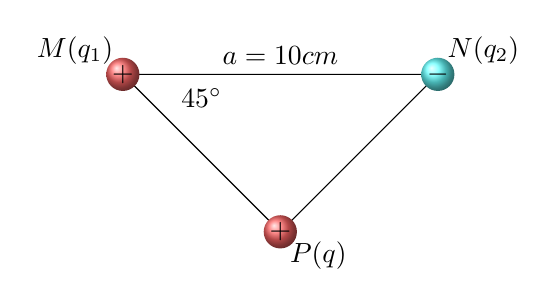
\begin{tikzpicture}[scale=1]
			\coordinate [label=above left:$M(q_{1})$] (M) at (-1.0cm,1.0cm);
			\coordinate [label=below right:$P(q)$] (P) at (1.0cm,-1.0cm);
			\coordinate [label=above right:$N(q_{2})$] (N) at (3cm,1.0cm);
			\draw (M) -- node[above] {$a=10cm$} (N) -- node[right] {$$} (P) -- node[below] {$$} (M);
			\tkzMarkAngle[size=.5cm,color=cyan,mark=|](P,M,N)
			\tkzMarkAngle[size=.5cm,color=cyan,mark=|](M,N,P)
			\shade[ball color=red!60] (M) circle (6pt);
			\node at (M) {$+$};
			\shade[ball color=cyan!60] (N) circle (6pt);
			\node at (N) {$-$};
			\shade[ball color=red!60] (P) circle (6pt);
			\node at (P) {$+$};
			\node at (0cm,.7cm) {$45^\circ$};
			\end{tikzpicture}
		\end{figure}
		\item ចំណុចបន្ទុកអគ្គិសនីបីត្រូវបានដាក់លើកំពូលនៃត្រីកោណសម័ង្សមួយ ដូចបង្ហាញក្នុងរូប។ 
		\begin{multicols}{2}
			គណនាកម្លាំងអគ្គិសនីផ្គួបដែលមានលើបន្ទុកអគ្គិសនី $7.00\mu C$។
			\begin{figure}[H]
				\centering
				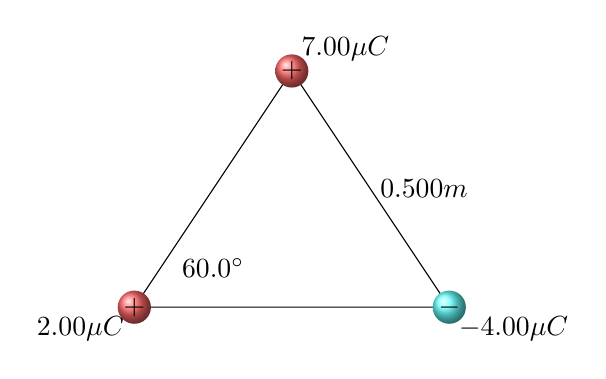
\begin{tikzpicture}[scale=1]
				\coordinate [label=below left:$2.00\mu C$] (M) at (-1.0cm,1.0cm);
				\coordinate [label=above right:$7.00\mu C$] (P) at (1.0cm,4cm);
				\coordinate [label=below right:$-4.00\mu C$] (N) at (3cm,1.0cm);
				\draw (M) -- node[above] {$$} (N) -- node[right] {$0.500m$} (P) -- node[below] {$$} (M);
				\tkzMarkAngle[size=.5cm,color=cyan,mark=|](N,M,P)
				\tkzMarkAngle[size=.5cm,color=magenta,mark=|](P,N,M)
				\tkzMarkAngle[size=.5cm,color=red,mark=|](M,P,N)
				\shade[ball color=red!60] (M) circle (6pt);
				\node at (M) {$+$};
				\shade[ball color=cyan!60] (N) circle (6pt);
				\node at (N) {$-$};
				\shade[ball color=red!60] (P) circle (6pt);
				\node at (P) {$+$};
				\node at (0cm,1.5cm) {$60.0^\circ$};
				\end{tikzpicture}
			\end{figure}
		\end{multicols}
		\item គេមានបន្ទុកអគ្គិសនី $Q,~-2Q,~3Q$ និង $-4Q$ ត្រូវបានគេយកទៅដាក់ត្រង់កំពូលនៃចតុកោណកែងមួយដែលមានវិមាត្រ $3a$ និង $4a$។
		\begin{multicols}{2}
			គណនាតម្លៃ និងទិសដៅនៃកម្លាំងផ្គួបដែលមានអំពើលើបន្ទុកអគ្គិសនី $Q$។
			\begin{figure}[H]
				\centering
				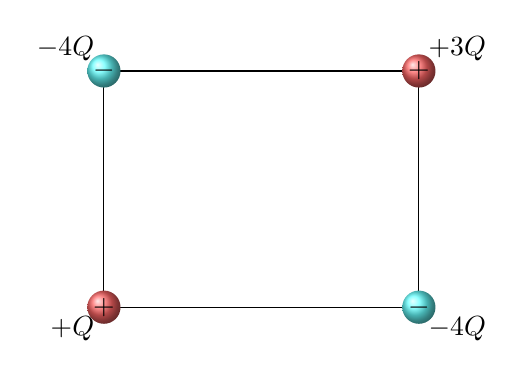
\begin{tikzpicture}
				\begin{scope}
				\coordinate [label=below left:$+Q$] (A) at (0.0cm,0.0cm);
				\coordinate [label=below right:$-4Q$] (B) at (4.0cm,0.0cm);
				\coordinate [label=above right:$+3Q$] (C) at (4.0cm,3.0cm);
				\coordinate [label=above left:$-4Q$] (D) at (0.0cm,3.0cm);
				\draw (A) rectangle (C);
				\shade[ball color=red!60] (A) circle (6pt);
				\node at (A) {$+$};
				\shade[ball color=cyan!60] (B) circle (6pt);
				\node at (B) {$-$};
				\shade[ball color=red!60] (C) circle (6pt);
				\node at (C) {$+$};
				\shade[ball color=cyan!60] (D) circle (6pt);
				\node at (D) {$-$};
				\end{scope}
				\end{tikzpicture}
			\end{figure}
		\end{multicols}
		\item គេមានបន្ទុកអគ្គិសនីបីដែលបន្ទុកអគ្គិសនីនីមួយៗ $Q$ ស្ថិតត្រង់កំពូលនៃត្រីកោណសម័ង្សមួយមានជ្រុង $a$។
		\begin{multicols}{2}
			គណនាអាំងតង់សុីតេ និងទិសដៅនៃកម្លាំងផ្គួបដែលមានអំពើលើបន្ទុកអគ្គិសនីមួយ។
			\begin{figure}[H]
				\centering
				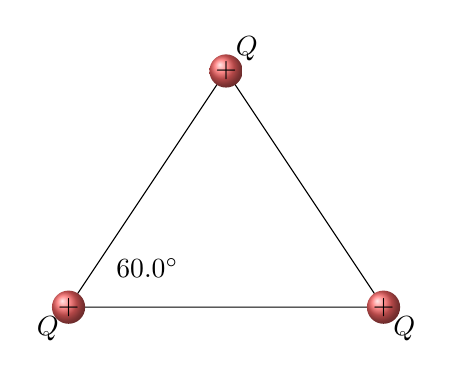
\begin{tikzpicture}[scale=1]
					\begin{scope}
						\coordinate [label=below left:$Q$] (M) at (-1.0cm,1.0cm);
						\coordinate [label=above right:$Q$] (P) at (1.0cm,4cm);
						\coordinate [label=below right:$Q$] (N) at (3cm,1.0cm);
						\draw (M) -- node[above] {$$} (N) -- node[right] {$$} (P) -- node[below] {$$} (M);
						\tkzMarkAngle[size=.5cm,color=cyan](N,M,P)
						\tkzMarkAngle[size=.5cm,color=cyan](P,N,M)
						\tkzMarkAngle[size=.5cm,color=cyan](M,P,N)
						\shade[ball color=red!60] (M) circle (6pt);
						\node at (M) {$+$};
						\shade[ball color=red!60] (N) circle (6pt);
						\node at (N) {$+$};
						\shade[ball color=red!60] (P) circle (6pt);
						\node at (P) {$+$};
						\node at (0cm,1.5cm) {$60.0^\circ$};
					\end{scope}
				\end{tikzpicture}
			\end{figure}
		\end{multicols}
		\newpage
		\item កូនបាល់បន្ទុកអគ្គិសនីឯកលក្ខណៈពីរត្រូវបានគេព្យូរទៅនឹងចំណុចនឹងមួយ ដោយខ្សែមិនយឺតនិងមិនគិតម៉ាសដែលមានប្រវែង $\ell=1.50m$ (ដូចរូប)។ បន្ទុកអគ្គិសនី $q=25.0\mu C$ ត្រូវបានបញ្ជួនទៅឲ្យកូនបាល់នីមួយៗ ក្រោយមកវាច្រានចេញគ្នាបានមុំ $25.0^\circ$ ជាមួយអ័ក្សឈរ។ តើម៉ាសរបស់កូនបាល់នីមួយមានតម្លៃប៉ុន្មាន?
		\begin{figure}[H]
		\centering
		\begin{tikzpicture}
		% save length of g-vector and theta to macros
		\pgfmathsetmacro{\Gvec}{1.5}
		\pgfmathsetmacro{\myAngle}{30}
		% calculate lengths of vector components
		\pgfmathsetmacro{\Gcos}{\Gvec*cos(\myAngle)}
		\pgfmathsetmacro{\Gsin}{\Gvec*sin(\myAngle)}
		
		\coordinate (centro) at (0,0);
		\coordinate (y) at (-1.5,-1.0);
		\coordinate (tension) at (-.6,-1.0);
		\node at (1,-1) {$\ell$};
		\node at (-1,-1) {$\ell$};
		\draw[dashed,magenta,-] (centro) -- ++ (0,-1.0) node (mary) [black,below]{$ $};
		\draw[thick] (centro) -- ++(270+\myAngle:3) coordinate (bob);
		\draw[thick] (centro) -- ++(270-\myAngle:3) coordinate (bob);
		\pic [draw, -, "$\theta$", angle eccentricity=1.5] {angle = bob--centro--mary};
		\pic [draw, -, "$\theta$", angle eccentricity=1.5] {angle = tension--bob--y};
		\draw [red, line width=2pt,-stealth] (bob) -- ($(bob)!\Gcos cm!(centro)$) node[ near end, right] {$\overrightarrow{T}$};
		\draw [green!50!black, line width=2pt,-stealth] (bob) -- ($(bob)!\Gsin cm!120:(centro)$)
		coordinate (gsin)
		node[near end, left] {$\overrightarrow{F}_{e}$};
		\draw [blue, line width=2pt,-stealth] (bob) -- ++(0,-\Gvec)
		coordinate (g)
		node[near end,right] {$\overrightarrow{F}_{g}$};
		%\pic [draw, -, "$\theta$", angle eccentricity=1.5] {angle = gcos--bob--g};
		\draw [dashed] (bob) -- (1.5,-2.5) node at (0,-2.5) [black, below] {$d$};
		\draw [dashed] (bob) -- (y);
		\shade [ball color=green!40] (bob) circle[radius=6pt];
		\shade [ball color=green!40] (1.5,-2.5) circle[radius=6pt];
		\fill[pattern = north east lines] ($ (centro) + (-.6,0) $) rectangle ($ (centro) + (.6,0.2) $);
		\draw [line width=2pt] (-.6,0) -- (.6,0);
		\end{tikzpicture}
	\end{figure}
	\end{enumerate}
\newpage
\section{ដែនអគ្គិសនី និងកម្លាំងអគ្គិសនី}